\roni{There is a bit of a mish-mash. 
Now you define MBD,then stop talking about it for a while 
and define BRP, then stop talking about BRP while
and talk about diagnoses, 
and then talk about BRP.
I recommend: say in the beginning that BRP is related to MBD. Then define MBD, diagnoses, MBDE and all that is not BRP. Only then define BRP properly.}

\section{Problem Definition}
In this section we define the batch repair problem and provide relevant background. 

%BRP is related to MBD

%MBD
Following standard model-based diagnosis (MBD) terminology, we denote by $\COMPS$ and $\OBS$ the components in the system and the observed system behavior, respectively. $\SD$ describes the behavior of the diagnosed system, and in particular the behavior of each component. The term {\em behavior mode} of a component refers to a state of the component that affects its behavior. $\SD$ describes for every component one or more behavior modes. For every component, at least one of the behavior modes must represent the nominal behavior of the component. The normal mode is often described by the clause $h(C_i) \rightarrow \varphi_{C_i}$, where $C_i\in \COMPS$. $h(C_i)$ is a predicate stating that $C_i$ is healthy, and $\varphi_{C_i}$ describes the nominal behavior of $C_i$. For instance, the nominal behavior of the lever valve (component $B$ in Figure \ref{fig:simple-example}) is to be opened once the float cage opens it, while an abnormal behavior can be stuck open or close.



A {\em batch repair problem} (BRP) arises when the assumption that all components are normal is not consistent with the system description and observations. Formally,
\[ \SD \wedge \OBS \wedge \bigwedge_{C\in \COMPS} h(C) ~~~ \text{is not consistent} \]





A mode assignment $\omega$ is an assignment of {\em behavior modes} to components. Let $\omega^{(+)}$ be the set of components assigned a nominal (i.e., normal) behavior mode and $\omega^{(-)}$ be the set of components assigned one of the other modes.


\begin{definition}[Diagnosis]
A mode assignment $\omega$ is called a diagnosis if $\omega \wedge \OBS \wedge \SD$ is satisfiable.
\end{definition}

In the example shown in Figure \ref{fig:simple-example}, assuming that all components are healthy under the observation that the water level is decreased is not consistent. Then a possible diagnosis is that components $A$, $C$ and $D$ are healthy, while $B$ is in an abnormal mode. For instance, the lever valve ($B$) is stuck close. 
Another possible diagnosis is that 
$B$, $C$ and $D$ are healthy, while $A$ is in an abnormal mode. In order to get the system to function correctly, at least one component must be repaired.

\begin{definition}[Repair Action]
A repair action can be applied to any subset of components and results in these components becoming normal. Applying a repair action to a set of components $\gamma$ is denoted by Repair($\gamma$).
\label{def:repairAction}
\end{definition}
\noindent ~\ref{def:repairAction} assumes that repair actions always succeed, i.e., a component is normal after it is repaired. %[Roni: TODO: discuss how to relax this assumption later in the paper.]

% What happens after a repair action
After a repair action, the system is tested to check if it has been fixed.
We assume that the system inputs in this test are the same as in the original observations ( $\OBS$ ). The observed system outputs are then compared to the expected system outputs of a healthy system. Thus, the result of a repair action is either that the system is fixed, or a new observation that may help choosing future repair actions.



% *** Define a diagnosis engine and what it returns ***
A model-based diagnosis engine (MBDE) accepts as input $\SD$, $\OBS$, and $\COMPS$ and outputs a set of diagnoses $\Omega$. Although a diagnosis is consistent with $\SD$ and $\OBS$, it may be incorrect. A diagnosis $\omega$ is {\em correct} if by repairing the set of components in $\omega^{(-)}$ the system is fixed. 
\roni{1. You use the term ``incorrect'' for a diagnosis, but only explain what is a ``correct'' diagnoses the sentence after. Reverse the order. 
2. I don't think your definition of ``correct'' is good, as it means that the diagnosis that contain all the components in the system is also ``correct''. 
I think in a ``correct'' diagnosis it also 
must be that no subset of it will result in a fixed system.}

Some diagnosis algorithms return, in addition to $\Omega$, a measure of the likelihood that each diagnosis is {\em correct}~\cite{williams2007conflict,abreu2011simultaneousDebugging,Stern15shely}. Let $p: \Omega \rightarrow [0,1]$ denote this likelihood measure. We assume that $p(\omega)$ is normalized so that $\sum_{\omega\in\Omega} p(\omega)=1$ and use it to approximate the probability that $\omega$ is correct.


% Light at the end of the tunnle
A common way to estimate the likelihood of diagnoses, assumes that each component has a prior on the likelihood that it would fail, denoted $p(c)$, and components fail independently ~\cite{Stern17shelly}. 
Under these assumptions, the likelihood of a diagnosis can be computed as
\begin{equation}
\displaystyle p(\omega)=\frac{\prod_{c\in\omega^{-}} p(c)}{\sum_{\omega'\in\Omega}{\prod_{c\in\omega'^{-}} p(c)}}
\label{eq:likelihoods}
\end{equation}
where the denominator is a normalizing factor. 
In our experiments we computed diagnoses likelihoods computed according to Equation~\ref{eq:likelihoods}, 
but other methods for computing likelihood of diagnoses also exist~\cite{mengshoel2010probabilistic} and the algorithms we propose are agnostic to how these probabilities are found. %$proposed algorithms .

% Repairing incurs a cost
Repairing a set of components incurs a cost, composed of a repair overhead and component repair costs. The repair overhead is denoted by $\cost_{repair}$, and the component repair cost of a component $c\in \COMPS$ is denoted by $\cost_{c}$.


\begin{definition}[Repair Costs]
Given a set of components $\gamma\subseteq \COMPS$, applying a repair action Repair($\gamma$) incurs a cost:
\[ \cost(Repair(\gamma)) = \cost_{repair} + \sum_{c\in \gamma} \cost_{c} \]
\end{definition}
We assume that all repair costs are positive and non-zero, i.e., $\cost_{repair}>0$ and $\cost_{c}>0$ for every component $c \in \COMPS$. As defined earlier, the task in BRP is to fix a system with minimum total repair cost.


As shown in Figure~\ref{fig:simple-example}, an efficient BRP solver should consider the possibility of repairing a set of components in a single repair action. Thus, the potential number of repair actions is %exponential in the number of components, in particular the power set of the components
$2^{|\COMPS|}$. Therefore, from a complexity point of view BRP is an extremely hard problem.


% *** Explain what is the sytem repair likelihood ***
\subsection{System Repair Likelihood}\label{sec:Repair_Likelihood}
If the MBDE returns a single diagnosis $\omega$ that is guaranteed to be correct, then the optimal solution to BRP would be to perform a single repair action: Repair($\omega^{-})$. %to repair exactly the components in $\omega$.
This, however, is rarely the case, and more often possibly a very large set of diagnoses is returned by diagnosis algorithms. This introduces uncertainty as to whether a repair action would actually fix the system. We define this uncertainty as follows:

\begin{definition}[System Repair Likelihood]
The System Repair Likelihood of a set of components $\gamma\subseteq \COMPS$, denoted \sysrep{$\gamma$}, is the probability that Repair($\gamma$) would fix the system.
\end{definition}

Consider the relation between $p(\omega)$ and \sysrep{$\omega$}. If $\omega$ is correct, then repairing all components that are faulty, meaning $\omega^{(-)}$, would fix the system. Therefore, the likelihood of repairing $\omega^{(-)}$ causing the system to be fixed is at least $p(\omega)$, i.e.,
\[ \sysrep{\omega^{(-)}}\geq p(\omega)  \]
Moreover, if $\omega$ is correct then repairing any superset of $\omega^{(-)}$ would also fix the system. Thus, $\sysrep{\omega^{(-)}}$ may be larger than $p(\omega)$.
On the other hand, repairing any set of components that is not a superset of $\omega^{(-)}$, as there would still be faulty components in the system.
Therefore, a repair action Repair($\COMPS '$) would fix the system if and only if $\omega^{*{(-)}}\subseteq \COMPS '$, where $\omega^*$ is the correct diagnosis.
While we do not know $\omega^*$, we can compute \sysrep{$\gamma$} from $\Omega$ and $p(\cdot)$:
\[ \sysrep{\gamma} = \sum_{\omega\in \Omega \wedge \omega\subseteq \gamma} p(\omega) \]
\sloppy{For example, in the boiler tank depicted in Figure~\ref{fig:simple-example}, there are two diagnoses, $\{A\}$ and $\{B\}$, such that $p(\{A\})=0.6$ and $p(\{B\})=0.4$. Thus, $\sysrep{\{A\}}$=0.6, $\sysrep{\{B\}}$=0.4, and $\sysrep{\{A,B\}}$=$p(\{A\})$+$p(\{B\})$=1.}

%----system state definition - can be taken from dx-2014 paper, section 3.4
\subsection{System State During Repair}
\label{sec:sysStateDuring}
Fixing a system involves potentially many repair actions. We use the term {\bf repair process} to refer to the process of applying these sets of repair actions until the system is fixed.
During the repair process, two sets are maintained. 
{\bf Repaired:} the set of components already repaired, 
{\bf Observed:} the set of observations, including $OBS$ as well as all the additional observations obtained after performing a repair action. 
We use the term {\bf system state} to refer to the values of Repaired and Observed at a given point in time during the repair process. For a given system state, we denote by $\overline{Repaired}$ as the set of components that were not repaired yet, i.e., $\overline{Repaired} = COMPS \setminus Repaired$. Following standard mathematical notation, we denote by $2^{\overline{Repaired}}$ as the set consisting of $\overline{Repaired}$ and any of its subsets. As there is no need to repair a component twice to fix the system, only repair actions that repair a set of components that is a member of $2^{\overline{Repaired}}$ should be considered.
%-------------





%\section{Additional Search Space Design Choices}
%\meir{this section is redundant. only the first para is important. I think that it is trivial that union based is better than power set, since we check diagnoses rather than components. therefore, i would present the union based at the beginning of the search, as the search space. I would not present power set at all. If you wan, you can present there (when describing the search space) the power set and then say that since we deal with multiple fault diagnosis rather than single fault, a node in the first level of the tree includes a diagnosis rather than a component.} 
%hilla: I agree, will do

%\subsection{Power set vs. Union based.}
%Above, we defined the search space as the space of all possible subsets of components. An alternative approach that was also proposed in previous work on BRP~\cite{stern2015implementing} is to consider the space of all possible unions of diagnoses. In this search space the root of the search is still an empty set of components, but the $i^{th}$ level of the search tree consists all subsets of components that are unions of $i$ diagnoses from $\Omega$. Thus, the first level in the tree is all subset of components that form a diagnosis. 

%This has the intuitive reasoning that at least one of these diagnoses is supposed to be true (according to the known observation), and thus a repair algorithm should try to aim for fixing the problem in the next repair action. This search space formulation is referred to as the {\em Union-Based Search} while the former formulation described earlier in the paper is referred to as the {\em Subset-Based Search}. 


%Thus, in this approach, we consider in the search for the best repair action which includes a set of components that are a union of at most $k$ diagnoses, where $k$ is a parameter. We set the diagnoses in a decreasing order of their likelihood (Equation \ref{eq:likelihoods}) and choose the first $k$ diagnoses. Thus we increase the probability of repairing faulty components. This approach is referred to as the {\bf Union-based search}. \meir{up to here it is a repeatition of the former para. from here it is redundant.} Experimentally, the union-based search approach yielded much better results than the powerset-based search and thus we only show results for it in the experimental results below.

%For both powerset-based search and union-based search, increasing $k$ results in a larger search space and consequently higher computational complexity. On the other hand, a large search space increases the range of repair actions considered, and thus higher $k$ can potentially find better repair actions. This provides an often desired trade off of computation vs. solution quality. This trend is observable in our experimental results below.

%new pessimistic:

%There is no consideration of the future mistakes and by that the previous estimations ignores the future wasted costs caused by redundant repair actions. That puts the "pessimistic" characteristic  of the Pessimistic FN cost estimation in question, and in order to correct that flaw we offer another change to the computation formula.
%We added to the Pessimistic Next State FN cost computation another important component - the Future False Positive costs (FFP). As can be deduced from the name, we compute the future FP costs, similarly to the FP described above, with the slightest change of using the Health state of the next state of the system. 
%add formula
%In conclusion, the resulted new Pessimistic FN costs is computed as follows: 

%We propose an additional wasted cost utility function in addition to the previously proposed optimistic and pessimistic functions. Both optimistic and pessimistic functions do not explicitly consider future false positive costs, i.e., the cost that will be wasted in the future when repairing components that should not have been repaired. 

%Thus, for a batch of components $\gamma$, we estimate the future false positive costs, denoted $cost_{FFP}(\gamma)$, as follows:
%\[cost_{FFP}(\gamma)=\sum_{C \notin \gamma} (1-F(C))\cdot cost(C) \] 
%The resulting wasted cost utility function, which we refer to as ``FFP enhanced'',  is given by:
%\begin{multline}
%C_{WC}=cost_{FP}(\gamma)+(1-\sysrep{\gamma}) \cdot (cost^p_{FN}(\gamma)+ cost_{FFP}(\gamma))
%\end{multline}
%We call this modified wasted cost function the ``FFP enhanced'' cost function.\footnote{It is also possible to have a similar function but use $cost^o_{FN}(\gamma)$ instead of $cost^p_{FN}(\gamma)$.}

%relax the computation done in each component so that a possible suboptimal but feasible solution is obtained.

%To summarize, we propose three utility functions from the wasted cost utility function family. A pessimistic wasted cost function, that uses $\widehat{cost}_{FP}$ and $cost_{FN}^p$ to estimate $cost_{FP}$ and $cost_{FN}$, an optimistic wasted cost function that uses $\widehat{cost}_{FP}$ and $cost_{FN}^o$, and a new pessimistic wasted cost function, "FFP enhanced". 
%\meir{i would rephrase it as follows: "To summarize, we presented two variations of the wasted cost utility function, one that does not consider the future false positive cost and one that does consider it. Both variations present two factors that affect the wasted cost utility function: (1) false positive cost, and (2) two alternatives of false negative cost (optimistic and pessimistic)."} 

\section{Experimental Results}


We evaluated the proposed batch selection algorithms on standard Boolean circuit systems. Figure \ref{fig:74181} presents a logic diagram of one of these systems, a known MSI chip called the 74181. It is an arithmetic logic unit (ALU) that provides thirty-two functions of two 4-bit variables. $\COMPS$ in this example include the Boolean gates in the ALU. $\SD$ is the behavior description of the components, for instance, the healthy behavior of an $\textit{OR}$ gate implies the ``$\textit{OR}$'' behavior while abnormal behaviors can be stuck at 1 or at 0. $\OBS$ includes the inputs and outputs of the ALU. A diagnosis states which gates are healthy and which are in a faulty mode. The batch repair algorithms propose a set of gates to fix.

\begin{table}\centering
{\small
\begin{tabular}{|l|r|r|r|r|}
\hline
 {\bf Name} & {\bf $|${\tiny \COMPS}$|$} & {\bf in} & {\bf out} & {\bf \#observations} \\
\hline
    74181  & 65    & 14   & 8    & 26 \\
    74182  & 19    & 9    & 5    & 25 \\
    74283  & 36    & 9    & 5    & 22 \\
\hline
    c432   & 160   & 36   & 7    & 23\\
    c499   & 202   & 41   & 32   & 22\\
    c880   & 383   & 60   & 26   &  30\\
\hline
\end{tabular}
\caption{The Benchmark suite: systems  {\small 74XXX} and
         {\small ISCAS-85}, and scenarios Feldman.}
\label{tab:systems}
}
\end{table}%

The standard Boolean circuits we used in our experiments are presented in Table \ref{tab:systems}. The systems {\small 74XXX}~\cite{Hansen99} are described in the first three rows, and additional three systems of {\small ISCAS-85} \cite{Brglez89} are described in the following three rows. Observations were selected randomly from Feldman et al.'s~\shortcite{feldman2010approximate} known benchmark.
To adapt these benchmark systems and observations to be an experimental infrastructure for batch repair algorithms we set the prior probability of each gate to be faulty to 0.01 and chose a single diagnosis for each observation to serve as the injected faults. This is needed to decide when the system is fixed. Note that this ``true'' diagnosis was chosen with probability proportional to its likelihood of being correct, computed according to the priors mentioned above under the standard assumption of fault independence. The component repair cost was set to 5, and we experimented with repair overhead ($cost_{repair}$) costs of 10, 15, 20, and 25.

%All batch repair algorithms used a simple MBDE based on exhaustive search to generate diagnoses. Diagnoses were generated in order of increasing cardinality, and halted after either all subset minimal diagnoses were found or a timeout of 15 minutes was reached. We did not use a more sophisticated MBDE as it is not the focus of this work. Note that the batch repair algorithms are applicable to any MBDE.

%------------from socs paper:
We evaluated the search algorithms on a standard diagnosis benchmark that represents a Boolean circuit systems. Details about these circuits are presented in Table \ref{tab:systems} and were published by~\cite{Hansen99} and~\cite{Brglez89}.  
Observations were selected randomly from Feldman et al.'s~\shortcite{feldman2010approximate} known benchmark.
To adapt these benchmark systems and observations to be an experimental infrastructure for batch repair algorithms we set the prior probability of each gate to be faulty to 0.01 and chose a single diagnosis for each observation to serve as the injected faults. This is needed to decide when the system is fixed. Note that this ``true'' diagnosis was chosen with probability proportional to its likelihood of being correct, computed according to the priors mentioned above under the standard assumption of fault independence. The component repair cost was set to 5, and we experimented with repair overhead ($cost_{repair}$) costs of 10 and 25.

All batch repair algorithms used a simple MBDE based on exhaustive search to generate diagnoses. Diagnoses were generated in order of increasing cardinality, and halted after either all subset minimal diagnoses were found or a timeout of 15 minutes was reached. We did not use a more sophisticated MBDE as it is not the focus of this work. 
In every experiment we run the evaluated algorithm to choose a batch repair action. Then performed this repair action. 
If the system is not fixed yet, then we run again the evaluated algorithm to choose the next batch repair action. This process continues until the system is fixed. The overall costs 
spent during this process is recorded. Since the \brps{} problem can be very difficult to solve, we limited the runtime of all algorithm to 5 minutes. 
An algorithm that reached this timeout was forced to return the incumbent solution. 
%%%%%%%%%%%%%%%%%%%%%%%%%%%%%%%%%%%%%%%%%%%

%We run the batch repair algorithms with different instances of fault injection on standard Boolean circuits presented in Table \ref{tab:systems}. The systems {\small 74XXX}~\cite{Hansen99} are described in the first three rows, and additional three systems of {\small ISCAS-85} \cite{Brglez89} are described in the following three rows. To adapt the Boolean circuits as an experimental infrastructure for batch repair algorithms we set the prior probability of each gate to be faulty to 0.01 and its repair cost to 5. Then, observations were selected randomly from Feldman et al.'s~\shortcite{feldman2010approximate} known benchmark, and a single diagnosis of these observations were selected as the true faults. A diagnosis was selected as the true fault with probability proportional to its likelihood of being correct, computed according to the priors mentioned above under the standard assumption of fault independence. Given an observation, all subset minimal diagnoses were found using exhaustive search. Note that the batch repair methods are indifferent to the diagnosis algorithms.  Also, we experimented with repair overhead ($cost_{repair}$) costs of 10, 15, 20, and 25.

%. An observation was generated by injecting faults to some gates and computing the outputs by propagating random inputs. We varied the number of injected faults in a range of 1--4.
%For lack of space we do not add details about the diagnosis algorithm since the main novelty of this paper is by proposing batch repair methods.

\begin{figure}{}%{4cm}
\begin{center}
  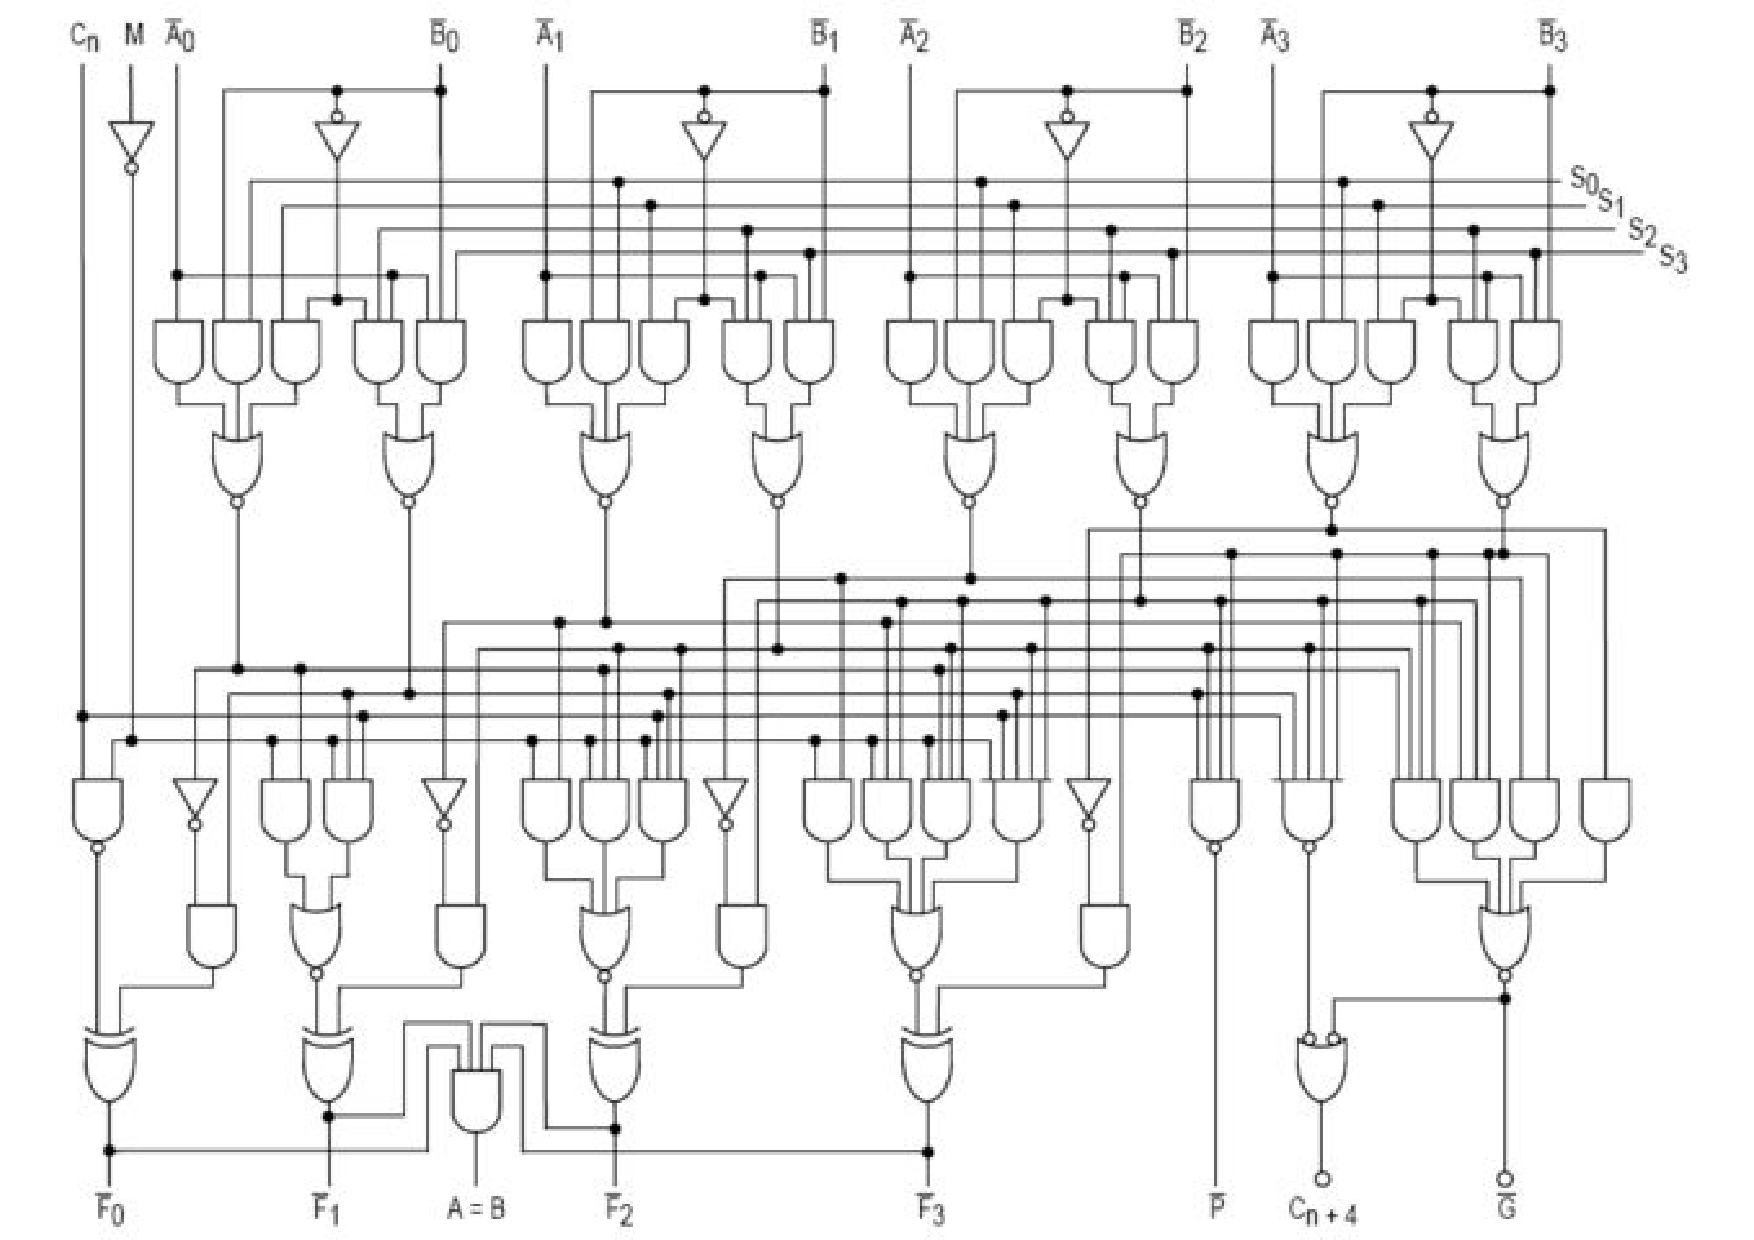
\includegraphics[width=0.9\columnwidth]{74181.pdf}
  \caption{A logic diagram of ALU 74181.}
  \label{fig:74181}
\end{center}
\end{figure}


\subsection{Baseline Repair Algorithms}
%The main hypothesis of this line of work is that performing a batch repair action can save repair costs. To evaluate if the proposed batch repair algorithms are able to do so, we compare them with two repair algorithms that do not consider batch repair actions. These baseline repair algorithms, named ``Best Diagnosis'' (BD) and ``Highest Probability'' (HP),  are inspired by previous work on test planning~\cite{zamir2014using} and work as follows. BD chooses to repair a single component from the most preferred diagnosis in $\Omega$ (that with the highest $p(\cdot)$ value). From the set of components in the most probable diagnosis, BD chooses to repair the one with the lowest repair costs. The HP repair algorithm chooses to repair the component that is most likely to be faulty, as computed by the system's health state ($F[\cdot]$).

The main hypothesis of this line of work is that performing a batch repair action can save repair costs. To evaluate if the proposed batch repair algorithms are able to do so we compare them with 1-HP, in which the component that is most likely to be faulty is repaired. A similar approach was used by previous work on test planning~\cite{zamir2014using}. Another baseline repair algorithm we evaluated experimentally is to repair all components of the most likely diagnosis in a single batch repair action denoted {\em Batch Best Diagnosis} (hereinafter, BD-batch).

%.\meir{I think that the next comment is confusing and adds nothing} Note that this algorithm, denoted {\em Batch Best Diagnosis}, ignores repair costs, and serves as an extreme alternative to the BD algorithm that repairs a single component from the most likely diagnosis.



\subsection{Results}

\begin{table*}[htb]
\centering
\scriptsize
%\begin{tabular}{@{}lp{0.05cm}p{0.05cm}p{0.05cm}p{0.05cm}|rrrr|rrrr|rrrr|rrrr|rrrr@{}}
%\begin{tabular}{@{}lp{0.2cm}p{0.2cm}p{0.2cm}p{0.2cm}p{0.2cm}p{0.2cm}p{0.2cm}p{0.2cm}p{0.2cm}p{0.2cm}p{0.2cm}p{0.2cm}p{0.2cm}p{0.2cm}p{0.2cm}p{0.2cm}p{0.2cm}p{0.2cm}p{0.2cm}p{0.2cm}p{0.2cm}p{0.2cm}p{0.2cm}p{0.2m}@{}}
\setlength{\tabcolsep}{5pt}
\resizebox{\textwidth}{!}{
\begin{tabular}{l|rrrr|rrrr|rrrr|rrrr|rrrr|rrrr}
\hline
System   & \multicolumn{4}{c|}{74182}                 & \multicolumn{4}{c|}{74283}                 & \multicolumn{4}{c|}{74181}                   & \multicolumn{4}{c|}{c432}                  & \multicolumn{4}{c|}{c499}                  & \multicolumn{4}{c}{c880}                     \\ \hline
Overhead & 10       & 15       & 20       & 25       & 10       & 15       & 20       & 25       & 10       & 15       & 20        & 25        & 10       & 15       & 20       & 25       & 10       & 15       & 20       & 25       & 10       & 15        & 20        & 25        \\ \hline
1-HP     & 82       & 110      & 137      & 164      & 106      & 142      & 177      & 213      & 119      & 159      & 199       & 239       & 60    & 80    & 100   & 120   & 41    & 55       & 69       & 83       & 144      & 191       & 239       & 287       \\
BD       & 59       & 73       & 88       & 103      & 81       & 101      & 122      & 142      & 92       & 115      & 137       & 160       & 83       & 109      & 135      & 161      & {\bf 28} & 36       & 45       & 53       & 95       & 123       & 151       & 178       \\
2-HP     & 62       & 78       & 94       & 109      & 85       & 107      & 128      & 149      & 85       & 107      & 128       & 149       & 47       & 59       & 71       & 83       & 32       & 40       & 49       & 51       & 90       & 109       & 127       & 145       \\
3-HP     & 57       & 69       & 81       & 93       & 77       & 93       & 108      & 124      & 83       & 99       & 116       & 132       & {\bf 44} & {\bf 53} & {\bf 62} & 72       & 30       & 37       & 44       & 46       & {\bf 87} & {\bf 102} & {\bf 117} & {\bf 131} \\
4-HP     & 58       & 69       & 79       & 90       & 78       & 91       & 104      & 117      & 82       & 96       & 110       & 124       & 47       & 55       & 63       & 72       & {\bf 28} & {\bf 34} & {\bf 40} & 62       & 117      & 151       & 186       & 220       \\
Opt. (1) & 56       & 69       & 83       & 97       & 70       & 89       & 108      & 125      & 76       & 95       & 113       & 131       & 50       & 65       & 79       & 94       & 33       & 43       & 52       & 62       & 117      & 151       & 186       & 220       \\
Opt. (2) & {\bf 54} & 65       & 71       & 82       & 68       & 82       & 95       & 103      & {\bf 75} & 91       & 107       & 121       & 51       & 63       & 73       & 84       & 33       & 41       & 49       & 52       & 114      & 147       & 179       & 207       \\
Pes. (1) & 58       & 69       & 81       & 97       & 68       & 89       & 109      & 128      & 77       & 95       & 111       & 129       & 51       & 65       & 76       & 88       & 33       & 43       & 52       & 62       & 118      & 153       & 187       & 225       \\
Pes. (2) & 56       & {\bf 58} & {\bf 64} & {\bf 73} & {\bf 65} & {\bf 73} & {\bf 83} & {\bf 91} & 76       & {\bf 90} & {\bf 102} & {\bf 110} & 51       & 61       & 63       & {\bf 69} & 32       & 40       & 45       & {\bf 49} & 118      & 149       & 178       & 205      \\ \hline
\end{tabular}
}
\caption{Average repair costs until system is fixed.}
\label{tab:cost-results}
\end{table*}



Table~\ref{tab:cost-results} shows the average repair costs incurred until the system was fixed for the systems and problem instances described above.
The first column lists the name of the compared algorithms, where $Opt.(\cdot)$ and $Pes.(\cdot)$ denote the union-based search using either pessimistic or the optimistic wasted costs utility functions, i.e., where
 $cost_{FN}^p$ and $cost_{FN}^o$ are used to estimate $cost_{FN}$, respectively, and the number in brackets (either 1 or 2) is the value of $k$. We did not experiment with larger values of $k$ due to computational complexity. 
The powerset-based search approach yielded substantially worse results compared to the union-based results so we do not display it in Table~\ref{tab:cost-results}.
The other columns in Table~\ref{tab:cost-results} show the results for different overhead costs -- 10, 15,20, and 25. For every system and column, we marked in bold the best performing algorithm for every combination of repair overhead cost and system.

%In our experiments these were the $k$-HP repair algorithm for $k=4$ and the union-based search repair algorithm for $k=2$ using either the pessimistic or the optimistic wasted costs utility functions (i.e., where  $cost_{FN}^p$ and $cost_{FN}^o$ are used to estimate $cost_{FN}$, respectively). These algorithms are marked in Table~\ref{tab:cost-results} by ``4-HP'', ``Pes. (2)'', and ``Opt. (2)''. We observed in both types of algorithms -- $k-HP$, $Pes. (k)$, and $Opt. (k)$ -- that increasing $k$ resulted in higher runtime and usually better results, but we  could not run larger values of $k$ in reasonable time.


The first trend we highlight is that in all cases, using a batch repair algorithm resulted in significantly less costs compared to the 1-HP, in which a single component is repaired in each round. This supports our main claim that reasoning about the possibility of batch repair is important. For example, in the 74181 system when the repair overhead is 25, 1-HP required an average cost of 239 while Pes.(2) needed only 110.  


Increasing the repair overhead causes all algorithms to require more cost to fix the system. However, the advantage of batch repair algorithms over 1-HP increase as repair overhead costs increases, demonstrating that the importance of batch repair is greater when overhead costs are higher. 

Also, in most cases the trivial BD-batch algorithm did not perform well, suggesting non-trivial algorithms are needed for intelligent use of batch repair. For example, in the c499 system with repair overhead of 25, BD-batch required an average cost of 161 while Pes.(2) needed only 69. No clear winner was observed when comparing the non-baseline approaches ($k$-HP, Opt.($k$), and Pes.($k$)), and in general most of these algorithms performed well. 
However, we do observe that in general Pes.($2$) is more robust in most system, being either the best performing or close to it in all systems except c880. 